\documentclass[journal,twoside,web]{ieeecolor}
\usepackage{jsen}
\usepackage{cite}
\usepackage{amsmath,amssymb,amsfonts}
\usepackage{graphicx}
\graphicspath{{../../results/figures/}{figures/}{./}}
\usepackage{textcomp}
\usepackage{wrapfig}
\usepackage{booktabs}
\usepackage{multirow}
\usepackage{url}
\usepackage{bm}
\usepackage{mathtools}
\usepackage{hyperref}
% ieeecolor already defines \proof, so amsthm is not loaded; LaTeX's own \newtheorem suffices.
\newtheorem{lemma}{Lemma}
\newtheorem{theorem}{Theorem}
\newtheorem{corollary}{Corollary}
% Public code + data repository (single source of truth)
\newcommand{\repourl}{https://github.com/Praveg432/OmniST}
\newcommand{\Risk}{r}
\markboth{\journalname, VOL. XX, NO. XX, XXXX 2026}
{Vashishtha: OmniST: Topology-Invariant Forecasting for Dynamic Sensor Networks}
\definecolor{abstractbg}{rgb}{0.89804,0.94510,0.83137}
\setlength{\fboxrule}{0pt}
\setlength{\fboxsep}{0pt}
\begin{document}
\title{OmniST: Topology-Invariant Forecasting for Dynamic Sensor Networks With Conformal Intervals at
Unseen Sensors}
\author{Praveg Vashishtha
\thanks{Manuscript submitted XX, 2026. This research did not receive any specific grant from funding agencies in the public, commercial, or not-for-profit sectors.}
\thanks{P. Vashishtha is with the Department of Computer Science and Engineering, Indian Institute
of Technology Patna, Patna 801106, India, and with Sopra Banking Software India, where he is a Senior
Software Development Engineer (e-mail: praveg\_pa2503mth259@iitp.ac.in).}}
\IEEEtitleabstractindextext{%
\fcolorbox{abstractbg}{abstractbg}{%
\begin{minipage}{\textwidth}%
\begin{wrapfigure}[12]{r}{3in}%
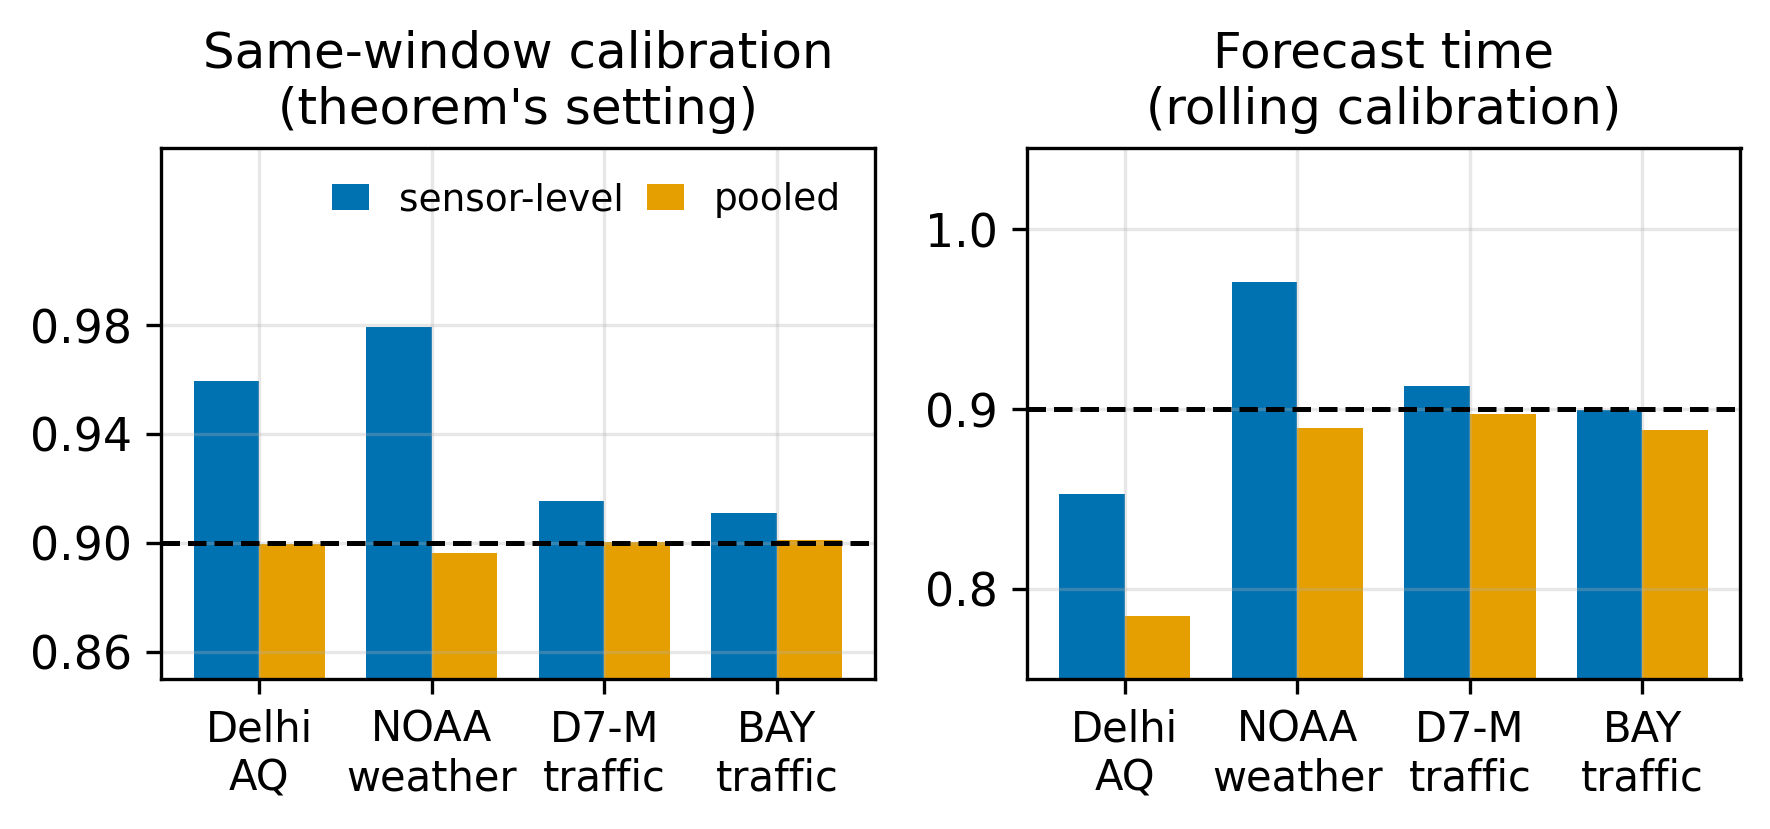
\includegraphics[width=3in]{graphical_abstract_jsen.png}%
\end{wrapfigure}%
\begin{abstract}
Deployed sensor networks change: stations are added, fail, or go offline, and forecasters built on a fixed adjacency matrix cannot forecast at a sensor added after training. We present OmniST, a forecaster with no dependence on the number of sensors, and ask when conformal intervals at a new sensor can be trusted. The usual recipe fails twice: calibration errors from training sensors are not exchangeable with errors at a new sensor, and the errors one sensor produces over time are dependent, so counting forecasts overstates the calibration set. When neighbors are drawn from the training network, a new sensor's error does not depend on other new sensors, and a correction counted in calibration sensors gives expected coverage of at least $1-\alpha$ at a randomly drawn new sensor, a case of hierarchical conformal prediction. On five real networks over repeated random sensor splits the bound held in every finite case, at 1.1 to 1.6 times the width of the pooled rule with 11 to 89 calibration sensors. That setting calibrates on the window it evaluates and cannot run at forecast time. With calibration restricted to earlier windows, rolling recalibration kept the sensor-level rule within 0.001 of the 0.90 target or above on three of four networks, but not on Delhi (0.85), and the pooled rule fell short on all four (0.79 to 0.90). A coordinate-free shared GRU matched OmniST's accuracy within about 2\%, and a coordinate-normalization defect in our earlier code is reported and fixed.
\end{abstract}
\begin{IEEEkeywords}
Conformal prediction, inductive prediction, sensor failure, sensor networks, spatiotemporal forecasting, uncertainty quantification.
\end{IEEEkeywords}
\end{minipage}}}
\maketitle
\section{Introduction}
\label{sec:introduction}
\IEEEPARstart{A}{n} operational sensor network rarely keeps the layout it was trained on. India's
Central Pollution Control Board adds air-quality stations every year~\cite{panja2026estgcn}, traffic
detectors fail, and weather stations go offline for maintenance. A forecaster serving such a network
has to keep working when a sensor disappears, and it has to produce a usable forecast, with an
honest statement of its uncertainty, at a sensor that was installed after the model was trained.

Spatiotemporal graph convolutional networks (STGCNs)~\cite{yu2018stgcn} forecast accurately on a
fixed network, but they encode it as a pre-computed $N\times N$ adjacency matrix. A sensor added after
training has no row or column in that matrix, so the model produces no forecast there, and removing a
trained sensor breaks the matrix product. Some implementations recompute the adjacency and can adapt,
but that is an engineering choice rather than something the formulation provides.

A point forecast at a new sensor is not enough for an operator, who also needs to know how far to
trust it. Split conformal prediction~\cite{vovk2005algorithmic,angelopoulos2023conformal} supplies
distribution-free intervals, but its guarantee depends on the calibration errors being exchangeable
with the error at the point being predicted. For a forecaster at a new sensor this is easy to get
wrong in two ways. If the calibration errors come from the sensors the model was trained on, they are
systematically different from the errors at a sensor it has never seen. And even with disjoint
calibration sensors, the thousands of errors one sensor produces over time are strongly dependent,
so the number of calibration \emph{points} overstates the information the calibration set carries.
The unit that can be exchangeable across a random choice of new sensor is the sensor.

This paper makes a design and an evidence contribution built around that observation.
\begin{enumerate}
\item \textbf{A forecaster with no dependence on the sensor count}
(Section~\ref{sec:architecture}): ``topology invariant'' in the sense that the model produces outputs for any
set of sensors.
\item \textbf{A coverage result with stated assumptions.} A locality lemma (Lemma~\ref{lem:locality}) shows that
a new sensor's error depends only on its own data and its nearest training-network neighbors. With it,
Theorem~\ref{thm:coverage} bounds expected coverage at a randomly drawn new sensor, with a correction counted in
calibration \emph{sensors}. The statistics are not new: the rule is that of hierarchical conformal
prediction~\cite{lee2023hcp} and the proof is the conformal risk control argument~\cite{crc2024}. The lemma alone
does not imply coverage, which the previous version of this work assumed.
\item \textbf{Evidence in two settings.} On five real networks, from models trained on disjoint sensors, we
measure the bound where it holds, with calibration errors from the window being evaluated, and where it would be
used, with calibration restricted to earlier windows (Section~\ref{sec:results}). We report its price, where it
is vacuous, where it fails at forecast time, and the per-sensor spread that marginal coverage hides.
\item \textbf{What the architecture contributes}, against like-for-like forecasting baselines, seasonal-naive
forecasting and a coordinate-free shared per-sensor model.
\end{enumerate}
%% ====================================================================
\section{Method}
\label{sec:architecture}

\subsection{An Architecture With No Global Sensor Count}

OmniST satisfies one invariant: for any sensor $i$ the output $f(i)$ depends only on sensor $i$'s own
data and a fixed-size neighborhood $\mathcal{N}_k(i)$, never on the full set of sensors present.

\textbf{Coordinate tokens.} Each observation becomes a token
\begin{equation}
\mathbf{z}_i(t) = f_{\text{MLP}}(\phi_i, \lambda_i) + f_{\text{time}}(t) + W_f \mathbf{x}_i(t),
\end{equation}
where $f_{\text{MLP}}:\mathbb{R}^2\to\mathbb{R}^d$ is a 3-layer MLP on centered latitude and longitude,
$f_{\text{time}}$ encodes calendar features with sinusoidal harmonics, and $W_f$ projects the raw
measurements. No other sensor enters $\mathbf{z}_i(t)$. The centering constants of
$f_{\text{MLP}}$ were fixed for Delhi; for the other regions the coordinate input lies far outside the
intended range, so the learned coordinate embedding is better read as a sensor-identity feature than
as a geographic one. Section~\ref{sec:ablation} measures how much it matters.

\textbf{Neighbor attention.} Spatial context comes from the $k$ geographically nearest sensors,
\begin{equation}
\mathbf{z}_i' = \text{LayerNorm}\Big(\mathbf{z}_i + \sum_{j \in \mathcal{N}_k(i)} \alpha_{ij} W_v \mathbf{z}_j\Big),
\end{equation}
with $\mathcal{N}_k(i)$ found by Haversine distance at every forward pass and $\alpha_{ij}$ the
multi-head attention weights with a learned distance bias. We use a single attention layer, so the
receptive field of a sensor is exactly $\mathcal{N}_k(i)$. In the \emph{reference-restricted} mode
used for every coverage experiment, $\mathcal{N}_k(i)$ is searched only among the sensors of the
training network, so sensors outside it never influence one another.

\textbf{Per-sensor temporal model and head.} A bidirectional GRU processes each sensor's sequence
independently, and a 2-layer MLP maps the final state to the forecast horizon. The model has
${\sim}315$K parameters at $d{=}128$ and is trained with AdamW, cosine annealing, early stopping on
training-network validation windows, and the Peaks-Over-Threshold loss of~\cite{panja2026estgcn}.

\textbf{What a new sensor needs.} The input to the model at a sensor is that sensor's own recent
history. OmniST therefore forecasts at a sensor that has no \emph{training} history but has at
least one input window of observations. It does not address a location with no data at all.

\subsection{Setting for Coverage at New Sensors}
\label{sec:setting}

Let $\mathcal{T}$ be the training network and $\hat f$ the model fitted on data from $\mathcal{T}$
alone, including early stopping and any hyperparameter choice. Let $\mathcal{R}$ be a set of further
sensors that were not used in any way during fitting, observed over an evaluation window shared by
all of them. For $i\in\mathcal{R}$ let $\hat y_{i,u}$ be the forecast at the $u$-th of $U$
(window, horizon-step) points, computed by $\hat f$ from sensor $i$'s own input history and the
histories of its $k$ nearest sensors in $\mathcal{T}$. The nonconformity score is
$s_{i,u}=|\hat y_{i,u}-y_{i,u}|$ and the interval is $[\hat y_{i,u}-q,\ \hat y_{i,u}+q]$ (clipped at
zero for non-negative quantities, which cannot change coverage). The miscoverage at sensor $i$ is
\begin{equation}
\Risk_i(q)=\frac{1}{U}\sum_{u=1}^{U}\mathbf{1}\{s_{i,u}>q\},
\end{equation}
a non-increasing, right-continuous function of $q$ with values in $[0,1]$.

\subsection{Locality and Sensor-Level Coverage}
\label{sec:theory}

\begin{lemma}[Locality]
\label{lem:locality}
Let $S\ni i$ be any set of additional sensors present alongside $\mathcal{T}$, and let neighbors be
searched in $\mathcal{T}$ only. The forecast $\hat y_i$ depends on $(\mathcal{T},S)$ only through the
coordinates and history of sensor $i$ and of the $k$ sensors of $\mathcal{N}_k(i;\mathcal{T})$.
Consequently $\hat y_i$ is unchanged if sensors of $S\setminus\{i\}$ are added or removed, or if
sensors of $\mathcal{T}$ outside $\mathcal{N}_k(i;\mathcal{T})$ are added or removed.
\end{lemma}
\begin{proof}
The token of a sensor is a function of its own coordinates, time features and measurements. With one
attention layer, the output at $i$ aggregates the values of exactly $\mathcal{N}_k(i;\mathcal{T})$
with weights computed from $i$'s query, those neighbors' keys and the distances to them, and there is
no normalization across sensors. The GRU and the head act on each sensor separately. Nothing uses the
number of sensors or a sensor index. Ties in distance are broken by a fixed rule. \end{proof}

The lemma says what a score is a function of. It does not say that scores at calibration sensors
and at a new sensor have the same distribution, and so by itself it gives no coverage statement:
a model typically fits the sensors it was trained on better than sensors it never saw. What it does
establish is the structure the theorem needs. Every sensor of $\mathcal{R}$ is scored by one and the
same function, and the score of a sensor does not depend on which other new sensors are present.
We check the lemma numerically in the released tests: scoring many new sensors in one pass equals
scoring each alone added to $\mathcal{T}$, to $10^{-5}$, for both the exact and the scalable
neighbor search.

\begin{theorem}[Sensor-level coverage]
\label{thm:coverage}
Fix $\mathcal{T}$ and $\hat f$, and let $\mathcal{R}$ contain at least $n+1$ sensors. Draw $J$
uniformly from $\mathcal{R}$ and, given $J$, a uniformly random $n$-subset $\mathcal{C}$ of
$\mathcal{R}\setminus\{J\}$. For $\alpha\in(0,1)$ let
\begin{equation}
\hat q(\mathcal{C})=\inf\Big\{q\ge 0:\ \frac{1}{n+1}\Big(1+\sum_{i\in\mathcal{C}}\Risk_i(q)\Big)\le\alpha\Big\},
\end{equation}
with $\inf\emptyset=\infty$. Then $\mathbb{E}\big[\Risk_J(\hat q(\mathcal{C}))\big]\le\alpha$, the
expectation being over the draw of $(J,\mathcal{C})$.
\end{theorem}
\begin{proof}
Let $A=\mathcal{C}\cup\{J\}$. It is a uniformly random $(n+1)$-subset of $\mathcal{R}$, and given $A$
the sensor $J$ is uniform on $A$. Fix $A$. For $j\in A$ let $\hat q_{-j}$ be the threshold computed from
$A\setminus\{j\}$, and let $\tilde q=\inf\{q:\frac{1}{n+1}\sum_{i\in A}\Risk_i(q)\le\alpha\}$. The set
is non-empty because every $\Risk_i$ is zero beyond the largest score, and each $\Risk_i$ is
right-continuous, so the infimum is attained. Since $\Risk_j\le 1$,
\[
\tfrac{1}{n+1}\textstyle\sum_{i\in A}\Risk_i(q)\ \le\ \tfrac{1}{n+1}\big(1+\sum_{i\in A\setminus\{j\}}\Risk_i(q)\big)\quad\text{for all }q,
\]
so every $q$ admissible for $\hat q_{-j}$ is admissible for $\tilde q$, and $\hat q_{-j}\ge\tilde q$.
As $\Risk_j$ is non-increasing, $\Risk_j(\hat q_{-j})\le\Risk_j(\tilde q)$. Averaging over $j\in A$,
\[
\mathbb{E}\big[\Risk_J(\hat q(\mathcal{C}))\mid A\big]=\tfrac{1}{n+1}\textstyle\sum_{j\in A}\Risk_j(\hat q_{-j})
\le\tfrac{1}{n+1}\sum_{j\in A}\Risk_j(\tilde q)\le\alpha .
\]
Taking the expectation over $A$ completes the proof. \end{proof}

The argument is the conformal risk control argument~\cite{crc2024} with the per-sensor miscoverage
$\Risk_i$ as the loss. Because every sensor contributes the same number $U$ of points, the average
$\frac1n\sum_{i\in\mathcal{C}}\Risk_i(q)$ is the fraction of all pooled calibration errors above $q$,
so the rule is a pooled quantile with a different correction.

\begin{corollary}[Pooled form and price]
\label{cor:pooled}
Let $\alpha_n=(\alpha(n+1)-1)/n$. Then $\hat q$ is the $\lceil(1-\alpha_n)\,nU\rceil$-th smallest of the
$nU$ pooled calibration errors, and is infinite exactly when $n<1/\alpha-1$.
\end{corollary}
The usual split-conformal correction instead uses $(nU+1)$, that is $\alpha_{nU}\approx\alpha$, which
treats the $nU$ errors as exchangeable. Here the correction is counted in sensors: at $\alpha=0.1$ at
least $9$ calibration sensors are needed for a finite interval, $19$ at $\alpha=0.05$, and $4$ at
$\alpha=0.2$. This is the price of a distribution-free statement when sensors, not points, are
the exchangeable units. With the same number of points per sensor, the rule is exactly the threshold of
hierarchical conformal prediction~\cite{lee2023hcp}.

\textbf{What the theorem does and does not say.}
\emph{(A1) Random assignment.} The probability is over which sensor plays the new one. It is a
statement about a sensor drawn at random from $\mathcal{R}$, not about a named sensor, and not
conditional on location. If $\mathcal{R}$ is itself a random sample of a larger population of
sensors, the same bound holds over that population. A new sensor that is systematically different
from the calibration sensors, for instance far outside the network, is outside the theorem;
weighted conformal prediction~\cite{tibshirani2019covshift,barber2023nexcp} is the route there, and
Section~\ref{sec:distance} measures how much distance matters on our data.
\emph{(A2) Common window.} Calibration and test errors come from the same evaluation window. This is
the setting in which the theorem holds, and it cannot be run at forecast time: when a forecast for
window $t$ is issued, the calibration sensors' errors for window $t$ are not yet known. With
calibration restricted to earlier windows the errors of different windows are not exchangeable and the
theorem says nothing; Section~\ref{sec:deployable} measures what happens.
\emph{(A3) Independence of the model.} $\hat f$ is fitted without $\mathcal{R}$.
\emph{(A4) Own history.} Every sensor has its input window.
The bound is on average coverage over the $U$ points of a sensor, not per time step and not per sensor.

\textbf{Topology change.} Suppose a set $D\subset\mathcal{T}$ of reference sensors goes offline. By
Lemma~\ref{lem:locality} only the sensors of $\mathcal{R}$ with a neighbor in $D$ change their score;
the others keep theirs exactly. Recomputing the scores of the affected sensors against the reduced
reference network and recalibrating gives Theorem~\ref{thm:coverage} for the reduced network with the
same $\hat f$. The earlier version of this work claimed that no recalibration is needed in this case.
That is true only for the cached scores of unaffected sensors, not for the validity of a threshold
calibrated on a different network.

\subsection{Calibration at Forecast Time}
\label{sec:online-conformal}
Theorem~\ref{thm:coverage} is silent about calibration that uses only errors observed before the
forecast. For a forecast of window $t$ we consider four ways to form the threshold from the calibration
sensors' errors of earlier windows only: \emph{static} (windows before a fixed start $t_0$),
\emph{expanding} (all windows before $t$), \emph{rolling} (the previous $L$ windows), and \emph{ACI}
(rolling, with the working level updated from the new sensor's own realized miscoverage $e_t$ as
$\alpha_{t+1}=\mathrm{clip}\big(\alpha_t+\gamma(\alpha-e_t)\big)$, after Adaptive Conformal
Inference~\cite{gibbs2021aci}). Each is paired with the sensor-level or the pooled correction. None of
them carries a finite-sample guarantee here: ACI's long-run property is asymptotic and the horizons
are short, and the non-exchangeable conformal bounds~\cite{barber2023nexcp} would need a drift term
that we do not estimate. They are measured, and the settings $L$, $\gamma$, $t_0$ were fixed before
the results were seen.

%% ====================================================================
\section{Data and Evaluation Protocol}
\label{sec:experiments}

\subsection{Datasets}
We use five networks from three physical domains, all public.
\begin{itemize}
\item \textbf{Delhi air quality:} daily PM$_{2.5}$ from 37 CPCB stations (2019--2023), from the
E-STGCN repository~\cite{panja2026estgcn}. Training uses 2019--2022 except the last 180 days, which
form the validation set; the test year is 2023 (365 days), with 60-day inputs and a 30-day horizon.
\item \textbf{Beijing air quality:} hourly PM$_{2.5}$ from the 12-station UCI Multi-Site
dataset~\cite{zhang2017beijingair} (2013--2017), aggregated to daily; 30-day inputs, 15-day horizon.
\item \textbf{Western-US weather:} daily maximum temperature from 30 NOAA GHCN-Daily stations
(2018--2022) with native coordinates; 30-day inputs, 15-day horizon.
\item \textbf{Freeway traffic:} 5-minute speeds from the 228-sensor Caltrans PeMSD7-M
benchmark~\cite{yu2018stgcn} and the 325-sensor PeMS-BAY benchmark~\cite{li2018dcrnn}; 48-step inputs,
12-step horizon. Both release a distance adjacency, not coordinates, so positions are reconstructed by
classical multidimensional scaling. They are not physical coordinates.
\end{itemize}
Within each dataset the split is chronological: the last year (air quality, weather) or the last 20\%
(traffic) is the evaluation period, preceded by a validation block of 180 days or 10\%.
\textbf{Missing data.} Non-positive and implausible readings are treated as missing and filled by
forward fill, then backward fill, then the station median. Forecast targets in the evaluation period
may therefore contain imputed values, and no mask is used. Values are standardized with
training-network statistics.

\subsection{Random Sensor Splits}
\label{sec:splits}
Each experiment is repeated over independent random splits of the sensors into a training network
$\mathcal{T}$ and a held-out set $\mathcal{R}$, with a fresh model trained on
$\mathcal{T}$ for each split. All sensors of $\mathcal{R}$ are scored by the trained model in the
reference-restricted mode of Section~\ref{sec:architecture}, over the same evaluation windows. Windows
advance by the horizon, so target windows do not overlap; $U$ is the number of (window, horizon-step)
points per sensor. The unit of replication in every confidence interval below is the split, not the
forecast. Calibration and test sensors are then drawn \emph{from $\mathcal{R}$ at random inside each
split}, thousands of times, so that the expectation of Theorem~\ref{thm:coverage} is estimated directly
and without retraining.

Training/held-out sensors are 21/16 (Delhi), 6/6 (Beijing), 18/12 (weather), 168/60 (PeMSD7-M) and 235/90
(PeMS-BAY), over 10 splits for the first three networks and 4 for the traffic networks; the supplement lists
the windows, points per sensor and calibration sizes.

\subsection{Methods Compared}
All methods are evaluated at the sensors of $\mathcal{R}$ on identical windows, with identical
calibration. We separate three kinds of method, because they use different information.
\begin{itemize}
\item \textbf{Trained forecasters that use the sensor's own history and its training-network
neighbors.} \emph{OmniST} (coordinates, neighbor attention, GRU); \emph{No-attention}
(coordinates and GRU); and \emph{Coordinate-free} (a GRU shared across sensors, with neither
coordinates nor attention). The last is the control that shows what the spatial components add: it is
also inductive, since it has no sensor-specific parameters.
\item \textbf{Forecasters with no training.} \emph{Persistence} (last observed value) and
\emph{window mean} (mean of the input window), both from the sensor's own history only.
\item \textbf{Concurrent-observation interpolators (nowcasting references).} \emph{Nearest
neighbor} and \emph{inverse-distance weighting} predict the sensor from the values that training-network
sensors report \emph{during the target window}. A forecaster does not have these values at the
forecast origin, so these methods solve an easier task and are included as a reference, not as a
competitor. The previous version of this work compared OmniST with such interpolators, and with a
kriging network that reconstructs concurrent signals, as if the tasks were the same.
\end{itemize}

\subsection{Calibration Rules and Metrics}
Intervals are symmetric, $\hat y\pm q$. We compare the \emph{sensor-level} rule of
Theorem~\ref{thm:coverage} (Corollary~\ref{cor:pooled}) with the \emph{pooled} rule, the usual
split-conformal quantile with the $(nU+1)$ correction. Both are computed from the errors of $n$
calibration sensors, in two settings. In the \emph{same-window} setting the calibration errors are those
of the window being evaluated; it is the setting of the theorem and a reference, not a deployable
procedure. In the \emph{forecast-time} setting only errors of earlier windows, and the new sensor's own
realized errors, may be used: static, expanding, rolling ($L=4$ windows for the daily networks, 24 for
the 5-minute traffic networks) and ACI ($\gamma=0.1$), evaluated from window $L$ onward. Coverage is the fraction of the new sensor's points inside the interval,
averaged over random (new sensor, calibration set) draws; width is $2q$. Where $q=\infty$ the
interval is vacuous: coverage is 1 and the width is reported as infinite and excluded from width means.
Point accuracy is the mean absolute error over the sensors of $\mathcal{R}$. All intervals are
$t$-intervals over splits; differences between methods are paired within a split.

%% ====================================================================
\section{Results}
\label{sec:results}

\subsection{Does the Sensor-Level Bound Hold? Same-Window Calibration}
\label{sec:bound}

This subsection is the setting of Theorem~\ref{thm:coverage}: the calibration sensors' errors are those of the window being evaluated. It is a reference for what the theorem delivers, not a deployable procedure; Section~\ref{sec:deployable} removes that advantage.

Table~\ref{tab:bound} compares the two calibration rules at the 90\% target. For each trained model
we draw 4000 random (new sensor, calibration set) assignments from $\mathcal{R}$ (1500 for the two
traffic networks) and average the new sensor's coverage; the table gives the mean over splits.
Where Theorem~\ref{thm:coverage} gives a finite interval, its average coverage is at or above 0.90 in
every case, from 0.911 (PeMS-BAY, $n{=}89$) to 0.9996 (Delhi, $n{=}9$). The same holds at the 80\%
target (0.810 to 0.888 with at least 9 calibration sensors; the full set is in the released analysis
file). This is what the theorem predicts, and it is conservative: the guarantee costs width.

\begin{table}[htbp]
\caption{Coverage and Width at the 90\% Target, Sensor-Level Rule Versus Pooled Rule}
\label{tab:bound}
\centering
\footnotesize
\setlength{\tabcolsep}{3pt}
\begin{tabular}{lrcccccc}
\toprule
 & & \multicolumn{2}{c}{\textbf{Sensor-level}} & \multicolumn{2}{c}{\textbf{Pooled}} & \textbf{Width} & \textbf{Draws} \\
\textbf{Dataset} & $n$ & Cov. & Width & Cov. & Width & \textbf{ratio} & \textbf{$<0.80$} \\
\midrule
Delhi AQ   &  9 & 0.9996 & 491 & 0.8998 & 127.6 & 3.85 & --- \\
           & 15 & 0.9597 & 204 & 0.8997 & 127.6 & 1.60 & 0\% \\
Beijing AQ &  5 & vacuous & $\infty$ & 0.9003 & 179.0 & --- & 0\% \\
Weather    &  9 & 0.9996 & 36.8 & 0.8960 & 20.3 & 1.82 & --- \\
           & 11 & 0.9795 & 27.8 & 0.8965 & 20.3 & 1.37 & 13\% \\
PeMSD7-M   & 20 & 0.9443 & 27.3 & 0.8987 & 17.6 & 1.55 & --- \\
           & 59 & 0.9155 & 20.1 & 0.9003 & 17.6 & 1.14 & 5\% \\
PeMS-BAY   & 20 & 0.9448 & 40.8 & 0.8983 & 19.4 & 2.10 & --- \\
           & 89 & 0.9110 & 21.3 & 0.9010 & 19.4 & 1.10 & 8\% \\
\bottomrule
\multicolumn{8}{p{0.93\columnwidth}}{\footnotesize Means over 10 splits (Delhi, Beijing, weather) or 4
(traffic); widths in the units of each dataset. $n$ is the number of calibration sensors. ``Draws
$<0.80$'' is the share of random assignments, under the pooled rule at the largest $n$, whose new
sensor was covered less than 0.80 of the time. With 6 held-out sensors (Beijing) the sensor-level rule
is vacuous at the 90\% target; at the 80\% target and $n{=}5$ it gives coverage 0.960 at width 310
against 0.801 at width 129 for the pooled rule.} \\
\end{tabular}
\end{table}

\begin{figure*}[!t]
\centering
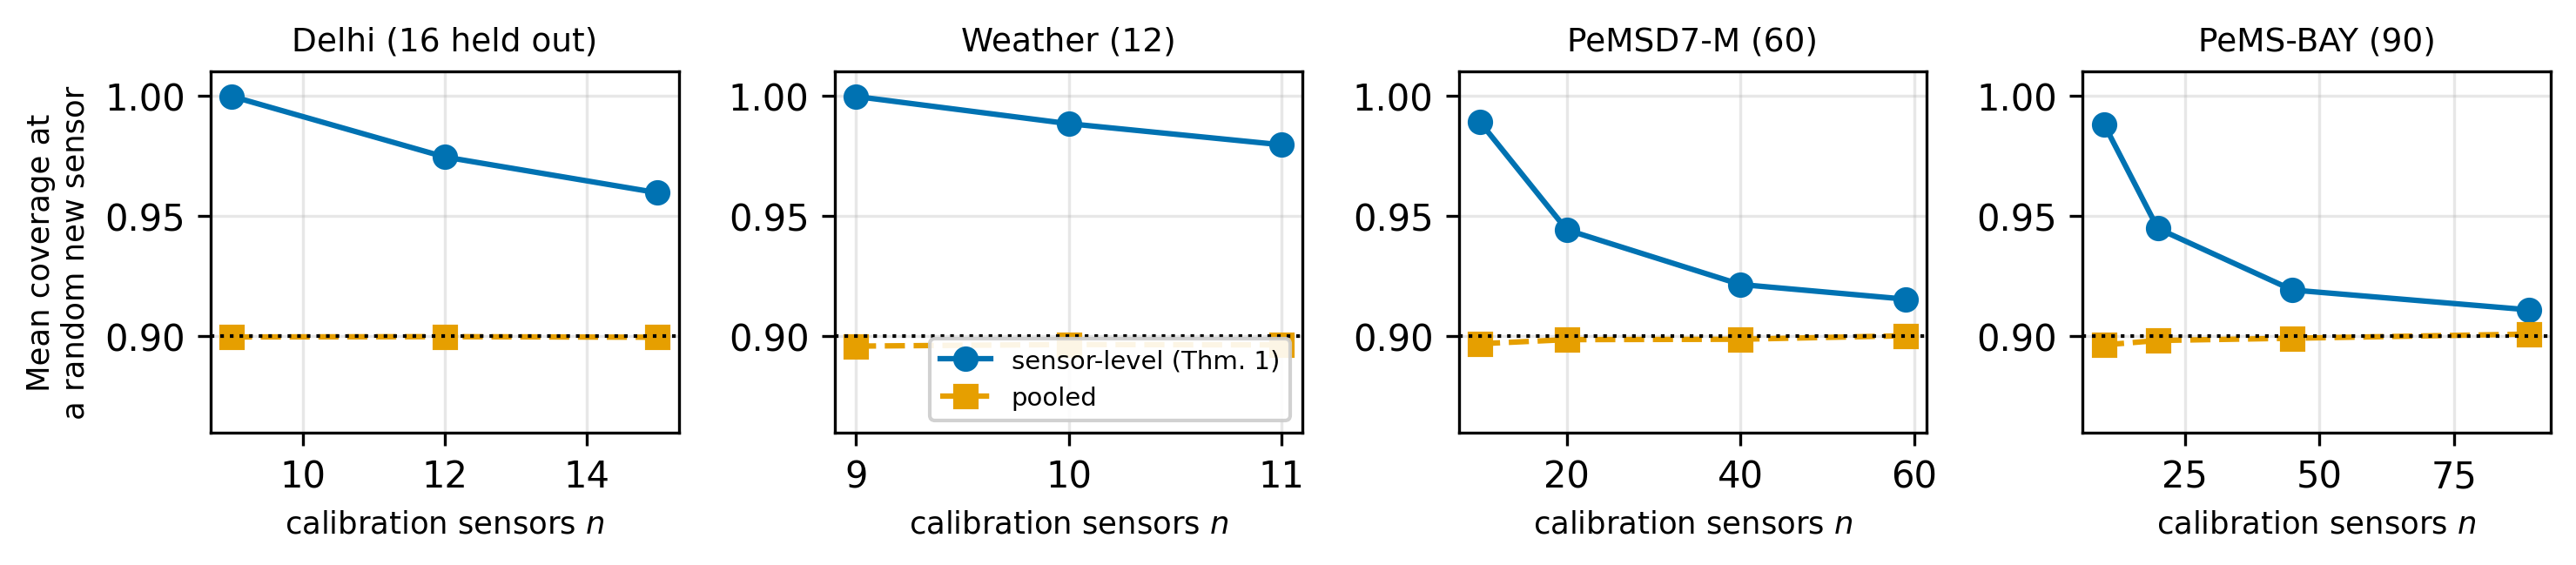
\includegraphics[width=0.72\textwidth]{fig_sensor_level.png}
\caption{Mean coverage as the number of calibration sensors grows, at the 90\% target (dotted line),
same-window calibration. The sensor-level rule stays above target and its price (Table~\ref{tab:bound}) falls as
$n$ grows; the pooled rule sits on the target on average.}
\label{fig:sensorlevel}
\end{figure*}

Three points follow. \emph{First}, the price is set by the number of calibration sensors and not by
the number of calibration points: with 9 to 15 sensors the interval is 1.4 to 4.3 times wider than the
pooled one, with 59 to 89 sensors it is 1.1 times wider. A network with a dozen held-out sensors cannot
support a finite distribution-free 90\% interval at all. \emph{Second}, the pooled rule, which has no
guarantee here, averages between 0.896 and 0.901 over random new sensors at every $n$ we tried. We read
this as an empirical fact about these networks, not as a property we can promise: in the weather data
it is 0.4 points under target, and the average hides the spread. For the same pooled rule, in 13\%
(weather), 8\% (PeMS-BAY) and 5\% (PeMSD7-M) of random assignments the new sensor is covered less
than 0.80 of the time, and the tenth percentile of the per-draw coverage is 0.78 to 0.88. Marginal
coverage is a statement about the average new sensor. \emph{Third}, nothing in Theorem~\ref{thm:coverage}
depends on OmniST: it applies to any forecaster whose error at a new sensor is a function of that
sensor's data and the training network, including the baselines below.

\subsection{Calibration at Forecast Time}
\label{sec:deployable}

Table~\ref{tab:deployable} repeats the evaluation with the threshold for each window formed only from
errors of earlier windows (Section~\ref{sec:online-conformal}), at the largest calibration size of each
network and the 90\% target. The same random (new sensor, calibration set) draws are used for every scheme.

\begin{table*}[!t]
\caption{Coverage at Forecast Time (Target 0.90). Static, Expanding, Rolling and ACI Calibration, Sensor-Level and Pooled Rules, Largest $n$}
\label{tab:deployable}
\centering
\footnotesize
\setlength{\tabcolsep}{5pt}
\begin{tabular}{lrlcccccc}
\toprule
 & & & \multicolumn{4}{c}{\textbf{Mean coverage}} & \multicolumn{2}{c}{\textbf{Share of draws $<0.80$}} \\
\textbf{Dataset} & $n$ & \textbf{Rule} & Static & Expanding & Rolling & ACI & Rolling & ACI \\
\midrule
Delhi AQ   & 15 & Sensor-level & 0.848 & 0.863 & 0.853 & 0.855 & 0.10 & 0.02 \\
           &    & Pooled       & 0.800 & 0.795 & 0.785 & 0.790 & 0.55 & 0.53 \\
Weather    & 11 & Sensor-level & 0.948 & 0.970 & 0.971 & 0.947 & 0.02 & 0.00 \\
           &    & Pooled       & 0.854 & 0.882 & 0.889 & 0.863 & 0.13 & 0.19 \\
PeMSD7-M   & 59 & Sensor-level & 0.914 & 0.914 & 0.913 & 0.900 & 0.05 & 0.00 \\
           &    & Pooled       & 0.900 & 0.899 & 0.897 & 0.883 & 0.07 & 0.00 \\
PeMS-BAY   & 89 & Sensor-level & 0.870 & 0.890 & 0.899 & 0.899 & 0.04 & 0.00 \\
           &    & Pooled       & 0.854 & 0.877 & 0.889 & 0.887 & 0.12 & 0.00 \\
\bottomrule
\multicolumn{9}{p{0.9\textwidth}}{\footnotesize Means over splits (10 for Delhi and weather, 4 for traffic) of
the new sensor's coverage averaged over the evaluated windows. Evaluation starts at window $L$: 6 windows for
Delhi, 18 for weather, 183 for PeMSD7-M and 116 for PeMS-BAY. Rolling uses $L=4$ windows (daily networks) or 24
(traffic); ACI uses $\gamma=0.1$. No theorem covers these schemes.} \\
\end{tabular}
\end{table*}

Four statements follow. \emph{First}, the same-window result is an upper bound on what the theorem-backed
procedure delivers at forecast time. With static calibration the sensor-level rule falls to 0.870 on
PeMS-BAY ($n{=}89$) and 0.848 on Delhi. \emph{Second}, rolling recalibration recovers the target on PeMS-BAY
(0.899) and keeps weather (0.971) and PeMSD7-M (0.913) above it, but not on Delhi, where no scheme exceeds
0.863. Delhi has six evaluation windows of 30 days and a strong seasonal cycle, and we do not claim the other
networks are free of drift. \emph{Third}, the pooled rule, which was on target in the same-window setting,
under-covers on Delhi, weather and PeMS-BAY under every scheme (0.785 to 0.889), and on PeMSD7-M it is within
0.003 of the target except under ACI (0.883). \emph{Fourth}, ACI removes the tail of badly covered sensors: the
share of random new sensors covered below 0.80 under the sensor-level rule falls from 10\%, 2\%, 5\% and 4\%
(rolling) to 2\%, 0\%, 0\% and 0\%. It does so by changing the width: relative to rolling, ACI intervals are 7\%
narrower on Delhi, 15\% on weather and 3\% on PeMSD7-M, and 31\% wider on PeMS-BAY (28.8 against 21.9). The
earlier version of this work reported that a rolling ACI layer raised late-year coverage on Delhi from 0.50 to
0.96. That result came from a different protocol and does not reproduce here; we withdraw it.

\subsection{What the Earlier Protocol Would Have Reported}
\label{sec:legacy}

The previous version of this work calibrated on the residuals of the training sensors and measured
coverage on 3 to 5 fixed held-out sensors, the same in every seed. It reported 0.914 to 0.928.
Table~\ref{tab:legacy} repeats the evaluation with sensors split at random into training,
calibration and test sets, over many splits (experiment C1, released with the code), once with disjoint
calibration sensors and once, on the same trained models, with training-sensor calibration. Mean
coverage is 0.876 to 0.906; three of five estimates lie below 0.90, and the earlier numbers were 1.3 to
3.9 points higher than the random-split means. On the same trained models, calibrating on training
sensors and calibrating on disjoint sensors differ by at most 0.018 in average coverage, in either
direction. The concern about exchangeability therefore did not turn into a large average error on
these data, but it remained unsupported until the sensor-level argument above.

\begin{table}[htbp]
\caption{Coverage Over Random Disjoint Sensor Splits (Target 0.90, Pooled Rule)}
\label{tab:legacy}
\centering
\footnotesize
\setlength{\tabcolsep}{3pt}
\begin{tabular}{lrccc}
\toprule
 & & \textbf{Disjoint cal.} & \textbf{Train-sensor} & \textbf{Worst} \\
\textbf{Dataset} & \textbf{Splits} & \textbf{(95\% interval)} & \textbf{cal.} & \textbf{sensor} \\
\midrule
Delhi AQ   & 20 & 0.893 [0.884, 0.901] & 0.901 & 0.777 \\
Beijing AQ & 20 & 0.903 [0.895, 0.912] & 0.902 & 0.861 \\
Weather    & 20 & 0.906 [0.881, 0.931] & 0.888 & 0.654 \\
PeMSD7-M   &  6 & 0.876 [0.843, 0.909] & 0.890 & 0.519 \\
PeMS-BAY   &  6 & 0.892 [0.872, 0.913] & 0.887 & 0.402 \\
\bottomrule
\multicolumn{5}{p{0.93\columnwidth}}{\footnotesize ``Worst sensor'' is the lowest per-sensor
coverage over all test sensors and splits, under disjoint calibration.} \\
\end{tabular}
\end{table}

\subsection{Accuracy at New Sensors and What Each Component Contributes}
\label{sec:ablation}

\begin{table}[htbp]
\caption{MAE at Held-Out Sensors, Mean Over Splits (95\% Interval)}
\label{tab:accuracy}
\centering
\footnotesize
\setlength{\tabcolsep}{3.2pt}
\begin{tabular}{lccccc}
\toprule
\textbf{Method} & \textbf{Delhi} & \textbf{Beijing} & \textbf{Weather} & \textbf{D7-M} & \textbf{BAY} \\
\midrule
OmniST (normalized)    & 28.5 & 48.8 & 4.75 & 3.66 & 4.49 \\
No attention           & 28.6 & 48.8 & 4.76 & ---  & ---  \\
Coordinate-free GRU    & 28.0 & 48.4 & 4.82 & 3.71 & 4.45 \\
Persistence            & 38.0 & 52.7 & 4.65 & 3.57 & 5.14 \\
Window mean            & 47.2 & 51.3 & 4.58 & 7.44 & 5.41 \\
OmniST, earlier code   & 28.0 & 49.6 & 5.72 & 9.76 & 5.17 \\
\midrule
IDW, concurrent$^\dagger$ & 18.9 & 8.4 & 3.22 & 7.63 & 5.66 \\
\bottomrule
\multicolumn{6}{p{0.93\columnwidth}}{\footnotesize Units of each dataset; D7-M is PeMSD7-M, BAY is
PeMS-BAY. ``Normalized'': coordinates normalized from the training network. ``Earlier code'' uses the
coordinate constants of the submitted version (see text). $^\dagger$Inverse-distance weighting of the
training sensors' \emph{concurrent} values: a nowcasting reference that a forecaster cannot use.} \\
\end{tabular}
\end{table}

Table~\ref{tab:accuracy} and the paired differences (95\% intervals over splits) lead to four
statements.

\emph{(i) Against no-training forecasters.} OmniST is clearly better than persistence on the
air-quality networks (Delhi $-9.5$ [$-10.8$, $-8.1$]; Beijing $-3.9$ [$-4.3$, $-3.5$]) and on PeMS-BAY
($-0.65$ [$-0.76$, $-0.55$]), and indistinguishable from it on weather ($+0.10$ [$-0.23$, $0.43$]) and
PeMSD7-M ($+0.09$ [$-0.19$, $0.37$]). On those two networks a forecaster that repeats the last value
is as accurate. The comparison with the concurrent-observation interpolators is not one of equals:
they see what happens at the neighboring sensors during the target window and they are better
on Delhi, Beijing and weather. We therefore withdraw the earlier statement that OmniST improves on
interpolation by 12\% and on a kriging network by 21\%, which compared a forecast with a
reconstruction.

\emph{(ii) The coordinate-free control.} A GRU shared across sensors, with neither coordinates nor
attention, is within about 2\% of OmniST on every dataset: OmniST minus control is $+0.57$ [$-0.20$, $1.33$]
on Delhi, $+0.42$ [$-0.02$, $0.87$] on Beijing, $-0.067$ [$-0.122$, $-0.012$] on weather, $-0.056$
[$-0.43$, $0.32$] on PeMSD7-M and $+0.04$ [$-0.03$, $0.11$] on PeMS-BAY. Removing only the attention
changes the error by at most 0.11 on the datasets where we ran it. \textbf{The capability to forecast
at a new sensor comes from sharing parameters across sensors, not from the coordinates or the
attention.} In the data we have, the coordinates and the attention do not improve accuracy at new
sensors; they make spatial context available, and the architecture keeps the locality property
that Lemma~\ref{lem:locality} needs, but we cannot claim a benefit from them.

\emph{(iii) A defect in the earlier code.} The coordinate embedding in the submitted version centered
and scaled coordinates with constants chosen for Delhi (latitude 28.6, longitude 77.1, scales 0.2 and
0.3). For any other region the input to the embedding MLP lay tens to hundreds of units outside its
intended range, and the control experiment exposed it: with those constants OmniST was 0.7 to 6.0
error units worse than the coordinate-free control on every dataset but Delhi (PeMSD7-M: 9.76 against
3.71). Normalizing coordinates with the mean and standard deviation of the \emph{training} network,
fixed before any held-out sensor is seen, removes the gap (PeMSD7-M: 3.66; weather: 5.72 to 4.75;
PeMS-BAY: 5.17 to 4.49). Delhi, whose range the constants were chosen for, is slightly worse after the
change ($+0.48$ [$0.24$, $0.73$]). Every coverage and accuracy result in this paper uses the
normalized version; Table~\ref{tab:accuracy} keeps the earlier values for the record.

\emph{(iv) Intervals are as wide as the forecaster is inaccurate.} The width of every interval follows
the error of its forecaster: persistence gives intervals about 1.5 times wider than OmniST on Delhi
and PeMS-BAY, and nearest-neighbor interpolation gives intervals about 2.9 times wider on PeMSD7-M, at
the same coverage.
Calibration, not the forecaster, is what makes the coverage hold.

\emph{(v) Against seasonal-naive.} A seasonal-naive forecast repeats the sensor's own value one period earlier
(a week for the daily networks, the previous day for the traffic networks), restricted for all methods to the
windows that have one. It is no better than persistence on Delhi and clearly worse than OmniST on Delhi
($-9.5$ [$-10.7$, $-8.3$], 10 of 10 splits) and Beijing ($-15.2$ [$-15.9$, $-14.5$]); it ties OmniST on weather
($-0.24$ [$-0.56$, $0.07$]) and is worse on PeMSD7-M ($-0.74$ [$-1.16$, $-0.32$]). On PeMS-BAY it is clearly better
than both learned models: MAE 3.56 against 4.68 for OmniST (OmniST minus seasonal-naive $+1.12$ [$0.95$, $1.30$],
0 of 4 splits), and its 90\% pooled interval is 15.6 wide against 20.5, so OmniST's intervals are 31\% wider.
\emph{(vi) Removing reference sensors} (30\% or 50\% of the training network at inference, rescoring and
recalibrating on the survivors) changes MAE by at most 0.6\% and coverage by about 0.3 points at most
(supplementary material). This is expected: the model reads only its $k$ nearest neighbors and, as the controls
show, gets little from them.

\subsection{Distance From the Training Network}
\label{sec:distance}

Assumption (A1) is least safe for a sensor far from the network. Holding out a contiguous region and relating
per-sensor coverage to the distance from the nearest training sensor, in units of the median spacing
(experiment C2), a distance effect appears only in the sparse weather network: coverage falls by 0.0136 per extra
spacing [$-0.0221$, $-0.0063$]. In the other four networks the within-sensor slopes lie within 0.004 of zero. A
total-variation bound on the shift between sensors' score distributions would be vacuous at our sample sizes
(experiment C3: median 0.11 on Delhi and 0.19 on weather, against a noise floor of 0.13). Weather is also where the
pooled rule most often misses badly for an individual sensor, but with one sparse network of 30 sensors this is a
pattern to test, not a result.

%% ====================================================================
\section{Related Work}
\label{sec:related}

\textbf{Dynamic and inductive forecasting.} Fixed-topology STGCNs~\cite{yu2018stgcn} couple weights to a sensor
count. Inductive kriging~\cite{ignnk2020} reconstructs the signal at unobserved locations from the concurrent
observations of other sensors, a different task from forecasting at a new sensor from its own history; our earlier
comparison with it is withdrawn. STFO~\cite{stfo2026} and cold-start forecasting at unseen
sensors~\cite{coldstart_unseen2026} target point prediction under growing networks. Our control
(Section~\ref{sec:ablation}) indicates that what these methods share, no sensor-specific parameters, is what makes
a model applicable at a new sensor. Inductive kriging protocols can leak spatial information through model
selection~\cite{yang2026leakagefree}; our splits keep held-out sensors out of fitting and early stopping.

\textbf{Conformal prediction on graphs, space and time.} Split
conformal prediction~\cite{vovk2005algorithmic,angelopoulos2023conformal} has been extended to correlated time
series~\cite{corel2025}, graph time series~\cite{conformalgraphts2026,incontextresidual2026}, dynamic and temporal
GNNs~\cite{validcpdyngnn2024,nonexchcptgnn2025}, stream networks~\cite{staci2025} and online Gaussian processes on
graphs~\cite{conformalgp_online2025}, mostly with a fixed node set. Zargarbashi and
Bojchevski~\cite{conformalinductivegnn2024} analyze the inductive case in which new nodes shift the scores of
message-passing GNNs. The locality of our architecture (Lemma~\ref{lem:locality}) removes that interference by
construction, but removing interference is not the same as establishing exchangeability.

The closest statistics treat grouped data. Hierarchical conformal prediction
(HCP)~\cite{lee2023hcp} gives distribution-free sets for a new observation from a previously unseen group. With the
same number of points per sensor, HCP's weighted quantile coincides exactly with the sensor-level rule of
Corollary~\ref{cor:pooled} (checked numerically in the released tests), so the rule itself is not new. What
differs is the statement: HCP states coverage for one observation of the new group and uses exchangeability within
the group to do so, whereas Theorem~\ref{thm:coverage} bounds the average over a sensor's points and needs only
exchangeability of sensors. Generalized HCP~\cite{mallick2026ghcp} also uses the first observations of the new
group, the situation of a sensor that has been running for a few windows; we have not evaluated it. Sequential
whitening~\cite{sen2026whitening} gives exact coverage under a correct working covariance, with a PM2.5
application, and model-free valid spatial prediction~\cite{validspatial2020} uses the random-location design that
our condition (A1) borrows. Non-exchangeable and covariate-shift
extensions~\cite{barber2023nexcp,tibshirani2019covshift} are the tools for new sensors that differ systematically
from the calibration sensors. What this paper adds is not a conformal method. It is the sensor-as-group view
applied to forecasting at new sensors, a locality property that makes sensor-level scores well defined, a
measurement of the guarantee's price, and a measurement of what is lost when calibration must respect forecast
time.

%% ====================================================================
\section{Limitations}
\label{sec:limitations}
\begin{itemize}
\item \textbf{The guarantee is on average over which sensor is new}, not for a named sensor (the worst
per-sensor coverage in Table~\ref{tab:legacy} is 0.40 to 0.86), a time step, or a sensor that differs
systematically from the calibration sensors. Real new sensors are not random draws.
\item \textbf{Its setting cannot be deployed.} At forecast time no theorem applies; the sensor-level rule with
rolling recalibration covered 0.853 on Delhi, and the deployable results rest on four networks and, for Delhi,
six evaluation windows.
\item \textbf{It is expensive with few calibration sensors}: a finite 90\% interval needs at least 9, and the
12-station Beijing network cannot support it.
\item \textbf{The pooled rule is not guaranteed}; its near-nominal same-window average is an observation on
five networks, with large per-sensor spread.
\item \textbf{The learned forecaster is not the best simple one everywhere.} Seasonal-naive forecasting
beats OmniST on PeMS-BAY (MAE 3.56 against 4.68, intervals 24\% narrower), persistence ties it on weather
and PeMSD7-M, and coordinates and attention add no measured accuracy. The training budget was fixed, not
tuned per variant.
\item \textbf{Related methods not evaluated}: Generalized HCP, HCP's second-moment variant, sequential
whitening, and other inductive forecasters under the forecasting task.
\item \textbf{Data and history.} Targets include imputed values; traffic positions are reconstructed from
distance matrices; architecture settings come from earlier Delhi development, so (A3) holds only up to that
history; a sensor with no history of its own is not handled; the largest network has 325 sensors.
\end{itemize}

%% ====================================================================
\section{Conclusion}
\label{sec:conclusion}
OmniST forecasts at sensors it never trained on and keeps working when reference sensors are removed.
The more durable result is about calibration. Conformal intervals at a new sensor need the sensor, not
the forecast, to be the exchangeable unit. With neighbors drawn from the training network, a new
sensor's error is a function of its own data and its neighbors alone (Lemma~\ref{lem:locality}), and a
correction counted in calibration sensors gives expected coverage of at least $1-\alpha$ at a randomly
drawn new sensor (Theorem~\ref{thm:coverage}). On five real networks the bound held in every finite
case, at a width cost that falls from several-fold to about 10\% as calibration sensors grow from 10
to 90. That setting calibrates on the window it evaluates. With calibration restricted to earlier
windows the guarantee no longer applies, and the sensor-level rule with rolling recalibration reached the
target on three of four networks but not on Delhi. The usual pooled rule averaged within half a point of
target in the same-window setting, left some new sensors badly under-covered, and fell short of target
at forecast time on three of four networks. Our controls say that the ability to forecast at a new sensor comes from sharing
parameters across sensors, and that coordinates and attention, in our implementation, add no measured
accuracy. Open problems are a coverage statement that survives calibration restricted to earlier
windows, coverage conditional on a sensor and on its distance from the network, and a fair comparison
with hierarchical conformal prediction and with other inductive forecasters. A tighter distribution-free
statement with few calibration sensors is unlikely: the conformal correction is tight up to a factor of
order $1/n$~\cite{crc2024}.

\section*{Data and Code Availability}
All datasets are public: Delhi CPCB PM$_{2.5}$ from the E-STGCN repository~\cite{panja2026estgcn};
Beijing Multi-Site Air Quality from the UCI repository~\cite{zhang2017beijingair}; western-US daily
temperature from NOAA GHCN-Daily; PeMSD7-M traffic from~\cite{yu2018stgcn}; and PeMS-BAY traffic
from~\cite{li2018dcrnn}. The implementation, including the model, loaders for every dataset, each
experiment script (the per-sensor score collection, the same-window and forecast-time coverage
analyses, and the random-split evaluation), the unit tests for Lemma~\ref{lem:locality}, a pinned environment, and an index mapping
each reported number to its result file, is available at \url{\repourl}.

\section*{Acknowledgment}
The author declares no competing interests; the work was carried out
independently of the author's employment at Sopra Banking Software India, which neither funded nor
directed it. During the preparation of this work the author used Kiro, an AI coding and writing
assistant, to help write and debug experiment code and to draft and edit the manuscript text. The
author reviewed and edited all such content and takes full responsibility for the article.

\bibliographystyle{IEEEtran}
\bibliography{../references}

\begin{IEEEbiographynophoto}{Praveg Vashishtha}
is pursuing the Executive M.Tech. degree in the Department of Computer Science and Engineering,
Indian Institute of Technology Patna, India, and is a Senior Software Development Engineer with Sopra
Banking Software India. His research interests include spatiotemporal forecasting for sensor
networks, uncertainty quantification, and regularization for kernel methods.
\end{IEEEbiographynophoto}
\end{document}


